\documentclass{article}

\usepackage{graphicx}
\usepackage{tikz}
\usepackage{tikzsymbols}
\usetikzlibrary{calc,patterns,shapes.geometric}
\pagestyle{empty}
\usepackage[margin=0pt]{geometry}
\geometry{papersize={14in,12in}}

\def\centerarc[#1](#2)(#3:#4:#5){\draw[#1] ($(#2)+({#5*cos(#3)},{#5*sin(#3)})$) arc (#3:#4:#5);}

\begin{document}
	\begin{figure}
		\centering
		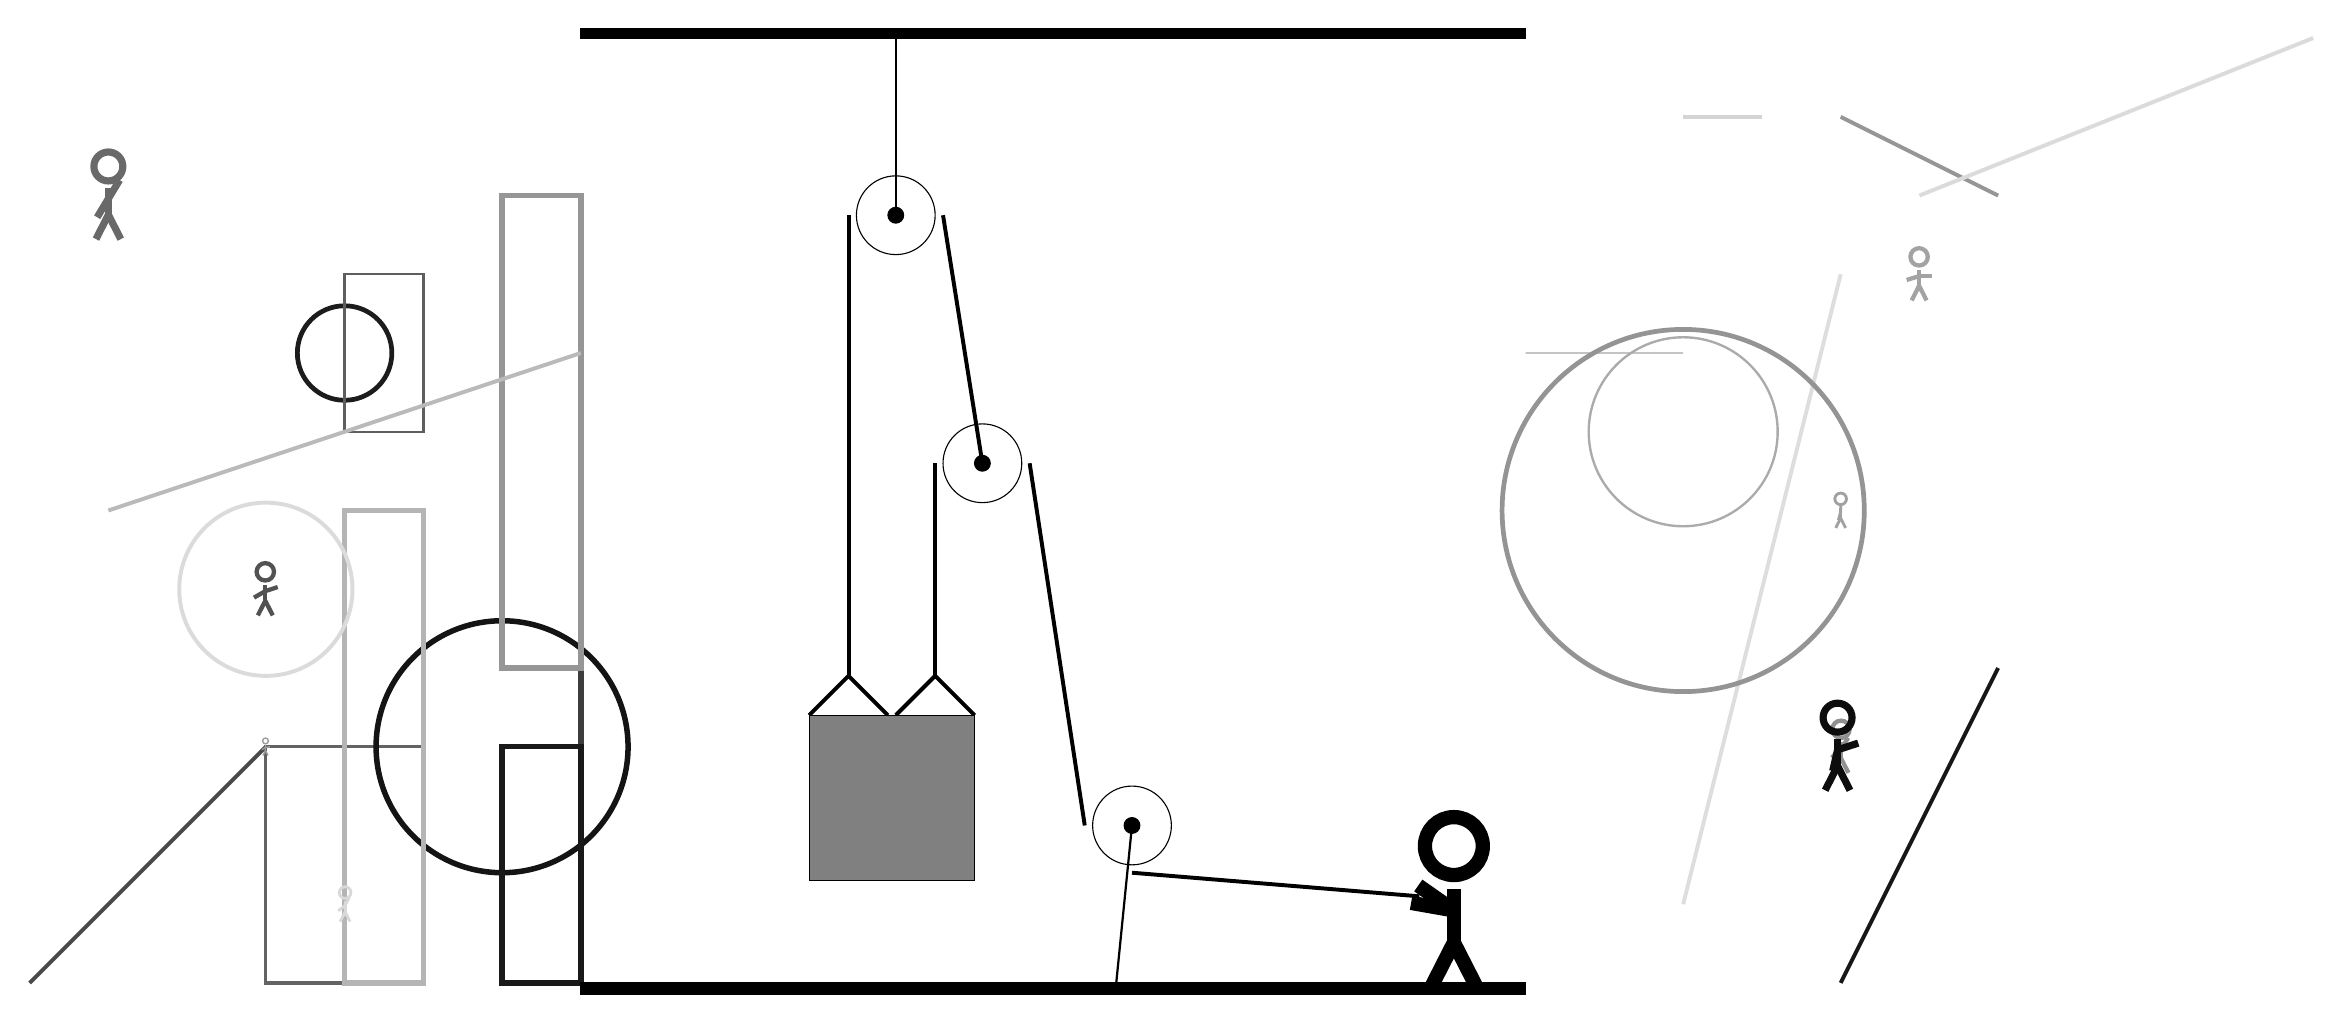
\begin{tikzpicture}
			%%%%% START %%%%%
			
			\draw[fill=black] (-2, 9) rectangle (10, 9.125);
			
			\draw (2, 6.75) circle (0.5);
			\draw[fill=black] (2, 6.75) circle (0.1);
			\draw[thick] (2, 6.75) -- (2, 9);
			
			\draw (3.1, 3.6) circle (0.5);
			\draw[fill=black] (3.1, 3.6) circle (0.1);
			
			\draw[line width=0.5mm, color=black!71](-6, 0) -- (-9, -3);
			
			\draw [line width=0.6mm, color=black!89](-5, 5) circle (0.6);
			\draw[line width=0.5mm, color=black!17] (12, 8) rectangle (13, 8);
			\draw[line width=0.7mm, color=black!76] (-2, 2) rectangle (-2, -2);
			
			\draw[line width=0.5mm, color=black!13](12, -2) -- (14, 6);
			
			\draw[line width=0.5mm, color=black!91](14, -3) -- (16, 1);
			
			\node[line width=0.3mm, color=black!36] at (15, 6) {\Strichmaxerl[3][17][0]};
			\draw[line width=0.4mm, color=black!61] (-4, -3) rectangle (-6, 0);
			\draw [line width=0.7mm, color=black!92](-3, 0) circle (1.6);
			\draw[line width=0.7mm, color=black!29] (-4, -3) rectangle (-5, 3);
			\draw[line width=0.2mm, color=black!23] (12, 5) rectangle (10, 5);
			\draw[line width=0.7mm, color=black!90] (-2, 0) rectangle (-3, -3);
			\node[line width=0.7mm, color=black!68] at (-6, 2) {\Strichmaxerl[3][30][18]};
			
			\node[line width=0.7mm, color=black!43] at (14, 0) {\Strichmaxerl[3][44][56]};
			\draw[line width=0.5mm, color=black!41](14, 8) -- (16, 7);
			\node[line width=0.7mm, color=black!95] at (14, 0) {\Strichmaxerl[5][77][18]};
			
			\draw [line width=0.3mm, color=black!33](12, 4) circle (1.2);
			\draw[line width=0.3mm, color=black!63] (-4, 6) rectangle (-5, 4);
			\node[line width=0.6mm, color=black!59] at (-8, 7) {\Strichmaxerl[5][59][59]};
			
			\draw[line width=0.7mm, color=black!41] (-2, 7) rectangle (-3, 1);
			\node[line width=0.2mm, color=black!15] at (-5, -2) {\Strichmaxerl[2][38][62]};
			
			\node[line width=0.2mm, color=black!38] at (-6, 0) {\Strichmaxerl[1][34][6]};
			\node[line width=0.3mm, color=black!37] at (14, 3) {\Strichmaxerl[2][75][89]};
			\draw[line width=0.5mm, color=black!27](-2, 5) -- (-8, 3);
			\draw [line width=0.5mm, color=black!14](-6, 2) circle (1.1);
			
			\draw [line width=0.6mm, color=black!42](12, 3) circle (2.3);
			\draw[line width=0.5mm, color=black!14](15, 7) -- (20, 9);
			
			\draw (5, -1) circle (0.5);
			\draw[fill=black] (5, -1) circle (0.1);
			\draw[thick] (5, -1) -- (4.8, -3);
			
			\draw[line width = 0.5mm]  (0.9, 0.4) -- (1.4, 0.9) -- (1.9, 0.4);
			\draw[line width = 0.5mm]  (2.0, 0.4) -- (2.5, 0.9) -- (3.0, 0.4);
			\draw[fill=black!50] (0.9, 0.4) rectangle (3.0, -1.7);
			
			\draw[line width = 0.5mm] (1.4, 6.75) -- (1.4, 0.9);
			\centerarc[line width = 0.5mm](2, 6.75)(0:180:0.6);
			\draw[line width = 0.5mm] (2.6, 6.75) -- (3.1, 3.6);
			\draw[line width = 0.5mm] (2.5, 3.6) -- (2.5, 0.9);
			\centerarc[line width = 0.5mm](3.1, 3.6)(0:180:0.6);
			\draw[line width = 0.5mm] (3.7, 3.6) -- (4.4, -1);
			\centerarc[line width = 0.5mm](5, -1)(180:270:0.6);
			\draw[line width = 0.5mm] (5, -1.6) -- (8.65, -1.9);
			
			\node at (9, -2) {\Strichmaxerl[10][-35][170]};
			
			\draw[fill=black] (-2, -3) rectangle (10, -3.15);
			
			%%%%% END %%%%%
		\end{tikzpicture}
	\end{figure}	
\end{document}